\section{L'erreur comme source de la connaissance scientifique}
\begin{myepigraph}
\og{}Les vraies révolutions sont lentes et elles ne sont jamais sanglantes.\fg{}\\[-1ex]
\normalfont{--- \citet{anouilh1956pauvre}}\\ 
\end{myepigraph}
\medskip
La science progresse en corrigeant constamment les erreurs,\smalltodo{progrès de science} c'est-à-dire que les erreurs précèdent nécessairement l'établissement de la connaissance scientifique. Bien que ce processus de correction des erreurs puisse être observé de manière diachronique, il est de nature circulaire. En outre, si une doctrine devient obsolète avec le temps et l'avènement des technologies avancées permettant de recueillir de nouvelles preuves, une doctrine actuellement en vigueur deviendra tout de même à son tour obsolète à un moment\footnote{L'un des exemples le plus connu de l'obsolescence scientifique est sans doute le passage du modèle géocentrique de l'univers, défendu par Aristote et Ptolémée (selon lesquels la Terre est immobile au centre de l'Univers), à la conception héliocentrique de Nicolas Copernic, qui affirmait que la Terre tournait autour du Soleil.}.

%\textit{doxa} (croyance)\footnote{Du grec ancien \textgreek{δόξα} signifiant \og{}opinion\fg{}.} d'hier devient \textit{épistémè} (connaissance)\footnote{Du grec ancien \textgreek{ἐπιστήμη} signifiant \og{}science\fg{}.} d'aujourd'hui, le dernier terme devenant à son tour doxa du lendemain, à la lumière de nouvelles preuves, et ainsi de suite\footnote{Dans \textit{République}, \textit{478}c, Platon oppose la \og{}croyance philosophique, doctrine\fg{} (\textgreek{δόξα}) à la \og{}science\fg{} (\textgreek{ἐπιστήμη}).}. 

Un tel cycle des observations empiriques peut être bouleversé, selon \citeauthor{bachelard1934formation} (\citeyear{bachelard1934formation}, p.~26), par la \og{}rupture et non pas continuité entre l'observation et l'expérimentation\fg{}. Autrement dit, la rupture épistémologique survient lors d'un renversement fondamental dans la façon d'établir une connaissance dans un domaine particulier. De fait, ce phénomène caractérise une \og{}révolution scientifique\fg{} \citep[p.~2]{koyre1957closed}, terme apparenté avec celui du \og{}changement de paradigme\fg{}\smalltodo{changement de paradigme}, introduit par \citeauthor{kuhn1962structure} (\citeyear{kuhn1962structure}, p.~66). D'après ce dernier, les \textit{paradigmes} désignent les \og{}découvertes scientifiques universellement reconnues qui, pour un temps, fournissent à une communauté de chercheur$\cdot$euse$\cdot$x$\cdot$s des problèmes types et des solutions\fg{}. 

\begin{multicols}{2}[\columnsep2.5em] 
\begin{figure}[H] % Use [H] to force the figure to stay in place
    \centering
    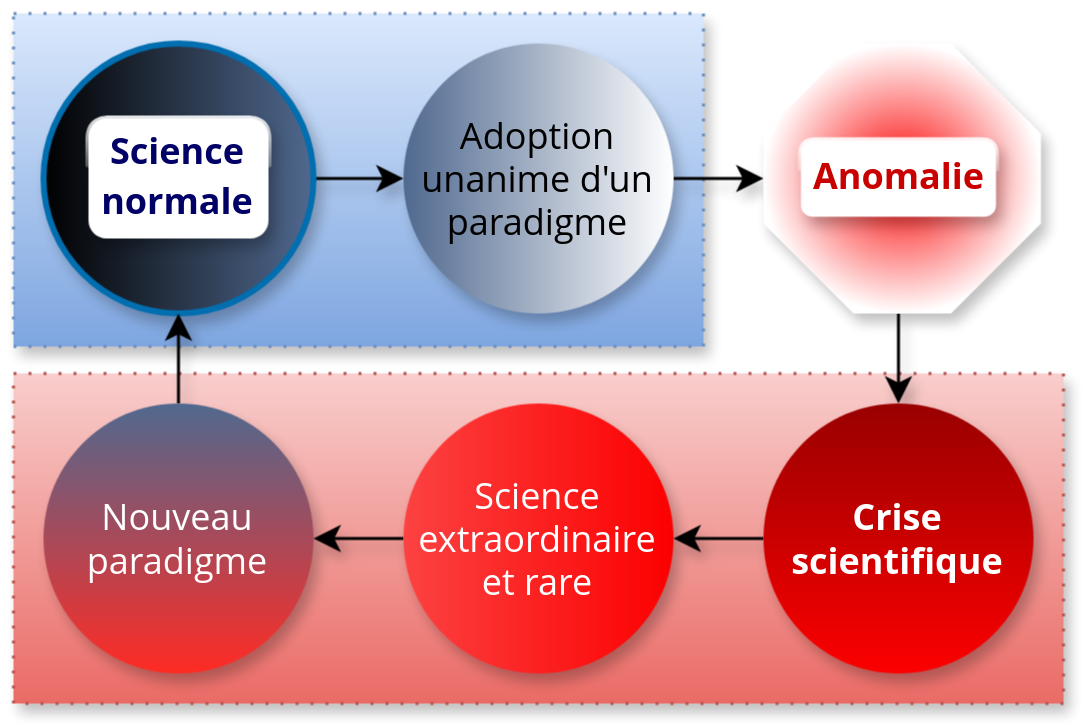
\includegraphics[width=\linewidth]{img/changement_paradigme.png}
    \caption{Conception kuhnienne du progrès scientifique, adaptée de \citet{amiri2012}.}
    \label{fig:changement_paradigme}
\end{figure}
\columnbreak

Dans cette optique, la structure des révolutions scientifiques désigne un modèle épistémique constitué des épisodes non cumulatifs \smalltodo{discontinuité} du développement scientifique (Figure \ref{fig:changement_paradigme}), marqués par des passages radicaux d'un paradigme à un autre.  Le nouveau paradigme ne désigne donc pas une extension de l'ancien paradigme ; au contraire, ce dernier est entièrement ou partiellement remplacé par un nouveau paradigme incompatible avec le précédent. \end{multicols} Cela est bel et bien un signe de l'\textit{émergence} d'une nouvelle théorie ou découverte, tout en prouvant que le développement historique des théories est fondamentalement discontinu. Dans un esprit similaire, \citeauthor{bachelard1970idealisme} (\citeyear{bachelard1970idealisme}, p.~72) souligne :

%\begin{figure}[h!]
%    \centering
%    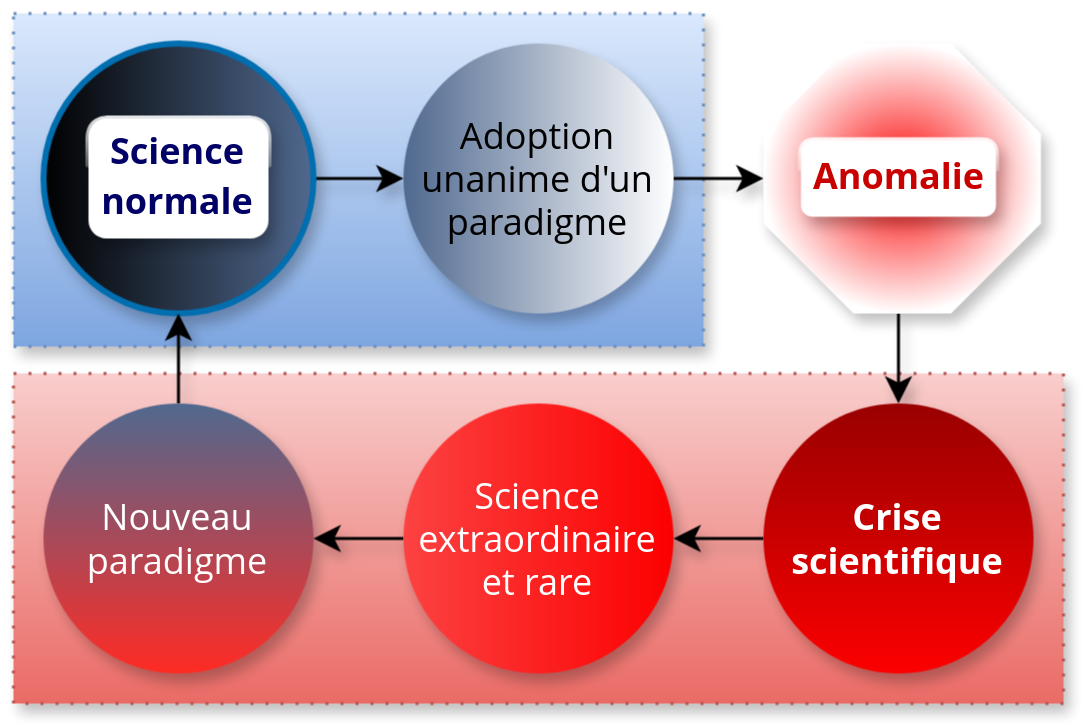
\includegraphics[width=75mm,scale=0.5]{img/changement_paradigme.png}
%    \caption{Conception kuhnienne du progrès scientifique, adaptée de \citet{amiri2012}.}
%    \label{fig:changement_paradigme}
%\end{figure}

%Un tel cycle des observations empiriques représente, selon \citet{koyre1962monde}, une \og{}révolution scientifique\fg{}, terme apparenté avec celui du \og{}changement de paradigme\fg{}, introduit par \citet{kuhn1983structure}. Dans cette optique, la structure des révolutions scientifiques désigne un modèle épistémique constitué des épisodes non cumulatifs de développement. Le nouveau paradigme ne désigne pas une extension de l'ancien paradigme ; au contraire, le dernier est entièrement ou partiellement remplacé par un nouveau paradigme incompatible avec le précédent, ce qui montre que le développement historique des théories est discontinu.
%
%Dans un esprit similaire, ce point épistémologique est relevé par \citet{bachelard1970idealisme} qui souligne :

\begin{quote} 

\og{}Il ne saurait y avoir de vérité \textit{première}. Il n'y a que des erreurs \textit{premières}.\smalltodo{erreurs premières} On ne doit donc pas hésiter à inscrire à l'actif du sujet son expérience essentiellement malheureuse. La première et la plus essentielle fonction de l'activité du sujet est de se tromper. Plus complexe sera son erreur, plus riche sera son expérience. L'expérience est très précisément le souvenir des erreurs rectifiées. L'être pur est l'être détrompé. \fg{} 
%\flushright{\cite{bachelard1970idealisme}} 
% \flushright{\cite[p.~89]{bachelard1970idealisme}} 

\end{quote}

%Un exemple de ce phénomène est l'évolution du terme \textit{hystérie} (associé exclusivement au sexe féminin jusqu'au XIX\ieme{} s.) dont l'histoire puise ses racines dans l'Antiquité, où cette maladie s'expliquait par un déplacement de l'uterus\footnote{Le terme \textit{hystérie} est issu du mot grec \foreignlanguage{greek}{ὑστέρα}, par le latin \textit{hystéra}, \og{}matrice\fg{}.}. Plus tard, à la fin du Moyen Âge, les hystériques étaient considérées comme possédées par le diable dans une perspective religieuse \citep{roudinesco}. Depuis les premières descriptions du cervelet faites de manière rigoureuse par Constanzo Varolio (1543-1575) à la Renaissance \citep{kneib2011etude}\footnote{Il s'agit des descriptions de la structure cérébrale, appelée \textit{pont} (lat. \textit{pons}) par Varolio (1573), puis \textit{pont de Varole} en l'honneur du célèbre anatomiste.}, suivies par la création du terme \textit{neurologia} par Thomas Willis (1621-1675) dans la période des Lumières en Angleterre, l'histoire de la neurologie trouve son ancrage au XIX\ieme{} siècle dans les travaux de Jean-Martin Charcot, considéré comme le père de la neurologie française et moderne (\citealp{teive2022thomas,BROUSSOLLE2012301}). Ce n'est qu'à cette période que la maladie en question a été traitée comme un trouble neurologique grâce à Charcot, selon qui l'hystérie découle d'une dégénérescence héréditaire du système nerveux \citep{tasca2012women}.

\label{hysterie} Un exemple du changement de paradigme est l'évolution du terme \textit{hystérie}, \smalltodo{évolution de l'hystérie} introduit par Hippocrate dans l'Antiquité au V\ieme{} s. av. J.-C., qui expliquait cette maladie par un déplacement de l'utérus dans le corps féminin\footnote{Ce terme est issu du mot grec \foreignlanguage{greek}{ὑστέρα}, par le latin \textit{hystera}, \og{}matrice\fg{}. Par dérivation, le terme hystérique se référait à une personne \og{}(femme) malade de l'utérus\fg{}, selon \citeauthor{rey2011dictionnaire} (\citeyear{rey2011dictionnaire}, p.~1767).}. Au Moyen Âge, surtout à partir du XIII\ieme{} s., les \textit{hystériques} étaient considérées par l'Église comme possédées par le diable et, par conséquent, chassées, torturées ou soumises aux exorcismes dans une perspective religieuse \citep[p.~113]{tasca2012women}. Néanmoins, certains scientifiques de la Renaissance commencent progressivement à s'éloigner de l'étiologie démonologique de cette maladie ; un cas notable est celui du médecin Charles Le Pois (1563-1633), qui fut le premier à désigner le cerveau, et plus précisément, le \textit{sensorium commune}\footnote{ce que \citeauthor{kant1863} (\citeyear{kant1863}, p.~452). appelle plus tard \og{}siège commun de la sensibilité\fg{} pour désigner l'ensemble des perceptions.}, comme siège de la maladie hystérique en 1618\footnote{\citeauthor{lepois1618} (\citeyear{lepois1618}, p.~101) a noté que les symptômes communément appelés hystériques se référaient à l'épilepsie, mais qu'il était prouvé que l'épilepsie elle-même était une maladie \textit{idiopathique} (existant par elle-même, sans lien avec une autre maladie) de la tête, et non pas provoquée par les troubles de l'utérus ou des intestins.}, en associant l'hystérie autant aux hommes qu'aux femmes \citep[p.~235]{wright1980}.  

Pour mieux comprendre l'importance de ce changement de pensée radical, il convient également de souligner que notre compréhension actuelle du système nerveux central est basée sur les premières descriptions faites de manière rigoureuse par Constanzo Varolio (1543-1575) au XVI\ieme{} s. \citep[p.~734]{tubbs2008costanzo}\footnote{Il s'agit de l'identification et de la description de la structure cérébrale agissant comme un relai entre le cerveau et le cervelet, appelée \textit{pont} (lat. \textit{pons}) par \citet{varolio1969nervis}, soit \textit{pont de Varole} (lat. \textit{pons Varolii}), en l'honneur du célèbre anatomiste, qui fut le premier à examiner le cerveau de sa base vers le haut.  
}. À l'époque des Lumières en Angleterre (fin XVII\ieme{} -- début XVIII\ieme{} s.), Thomas Willis (1621-1675), créateur du terme \textit{neurologia}\footnote{Terme présent dans \citet{willis1664cerebri}.} en 1664 \citep[p.~2]{monteiro2021}, maintint et développa cette conception en caractérisant cette maladie comme principalement convulsive en raison des explosions des \og{}esprits animaux\fg{} dans le cerveau \citep[p.~1]{willis1681essay}. Enfin, l'histoire de la neurologie trouve son ancrage à la fin du XIX\ieme{} siècle dans les travaux de Jean-Martin Charcot (1825-1893). Ce n'est qu'à cette période que la maladie en question a été systématiquement traitée comme un trouble neurologique \citep[p.~114]{tasca2012women}. \smalltodo{trouble cérébral}La sous-section \ref{JMC_polymathe} évoque certains de ses apports principaux dans le domaine scientifique.

\section{Jean-Martin Charcot : un médecin polymathe à l'aube de la neurologie moderne}
\label{JMC_polymathe}

Figure emblématique et directeur de l'illustre École de la Salpêtrière (basée à l'actuelle hôpital de la Pitié-Salpêtrière à Paris), Charcot a laissé une trace indélébile dans le domaine de la neurologie. 
Il est essentiellement connu pour ses études portant sur les troubles névrotiques, notamment l'hystérie. \smalltodo{contributions} Selon lui, l'hystérie découle d'une dégénérescence héréditaire du système nerveux \citep[p.~114]{tasca2012women}, en montrant qu'elle est en fait plus fréquente chez les hommes que chez les femmes. Charcot a été reconnu pour ses travaux de recherche sur l'hypnose qu'il a utilisée afin d'induire l'état modifié de conscience d'un sujet, permettant l'analyse des symptômes hystériques, ainsi que comme méthode de traitement. 
Son nom est également associé aux descriptions de nombreuses pathologies connues aujourd'hui, comme la \textit{maladie de Parkinson}, la \textit{sclérose en plaques disséminées}, abbr. \textit{SEP} (ou \textit{sclérose multiple}), la \textit{sclérose latérale amyotrophique}, abbr. \textit{SLA} (soit la \textit{maladie de Charcot}, ou \textit{maladie Lou-Gehrig}) etc\footnote{Pour un aperçu détaillé des contributions majeures de Charcot dans le domaine de la médecine, voir \citeauthor{camargo2024} (\citeyear{camargo2024}, p.~1102).}.

Ces explorations des abîmes de l'esprit humain lui ont valu de nombreuses appellations :\smalltodo{appellations} à part avoir été globalement considéré comme le père de la neurologie française et moderne (\citeauthor{teive2022thomas} \citeyear{teive2022thomas}, p.~761 ; \citeauthor{broussolle2012} \citeyear{broussolle2012}), d'autres noms plus symboliques lui ont été associés, notamment \og{}Napoléon des névroses\fg{}, \og{}Paganini de l'hystérie\fg{} \citep{mirbeau1995chroniques}, ou même \og{}César de la Faculté\fg{} \citep[p.~1109]{camargo2024}. Dans la même lignée de pensée, l'École de la Salpêtrière était caractérisée comme la \og{}Mecque de la neurologie\fg{} grâce aux activités de Charcot (\citeauthor{teive2014126} \citeyear{teive2014126}, p.~637 ; \citeauthor{GOETZ2017628} \citeyear{GOETZ2017628}, p.~628 ; \citeauthor{camargo2024} \citeyear{camargo2024}, p.~1100). En outre, de nombreuses références à Charcot et des descriptions d'attaques hystériques figurent non seulement dans la littérature médicale, mais aussi dans des romans\smalltodo{Charcot dans la littérature} naturalistes français et européens, notamment en Pays-Bas, Russie, pays scandinaves, Espagne, Italie et Allemagne \citep{KOEHLER201393}. 
%Il est essentiellement
%connu pour ses études sur les troubles névrotiques,
%notamment l'hystérie, la double personnalité, la catalepsie et le somnambulisme, ainsi que sur l'hypnose, méthode utilisée afin d'induire l'état modifié de conscience d'un sujet, permettant ainsi l'analyse des symptômes hystériques\footnote{Ces explorations des abîmes de l'esprit humain lui ont valu les appellations \og{}le Napoléon des névroses\fg{} ou bien \og{}le Paganini de l'hystérie\fg{} \citep{marmion2015freud}.}.

Charcot a créé un véritable réseau scientifique autour de soi grâce à ses idées novatrices \smalltodo{influences} qui ont eu un grand retentissement parmi ses collaborateurs, élèves et savants polymathes, dont nous ne nommons que quelques figures majeures souvent citées dans la littérature (\citeauthor{gomes2013jean} \citeyear{gomes2013jean}, p.~816 ; \citeauthor{bogousslavsky2014mysteries} \citeyear{bogousslavsky2014mysteries}, p.~55 ; \citeauthor{camargo2024} \citeyear{camargo2024}, p.~1100), notamment :
\begin{itemize}
\item Paul Richer (1849-1933), anatomiste, neurologue et sculpteur, qui a résumé les premières études de Charcot sur l'hystérie dans ses \textit{Études cliniques sur l'hystéro-épilepsie ou grande hystérie} ;
\item Georges Gilles de la Tourette (1857-1904), psychiatre et neurologue, qui a décrit les symptômes de la \textit{maladie des tics}, renommée \textit{syndrôme de Tourette} en son hommage par Charcot lui-même ;
\item Pierre Janet (1839-1916), philosophe, neurologue et psychiatre, concepteur des termes \textit{dissociation} et \textit{sous-conscient} ;
\item Désiré Magloire Bourneville (1840-1909), homme politique et neurologue, qui a publié le premier tome de l'ouvrage monumental l'\textit{Iconographie photographique de la Salpêtrière}, dédiée à l'hystérie, sous l'égide de Charcot ; 
\item Joseph Babinski (1857-1932), neurologue et neurobiologiste, concepteur du terme \textit{pithiatisme}, qui a découvert le réflexe cutané plantaire, appelé également \textit{signe de Babinski}.
\end{itemize}
\bigskip
L'impact colossal de Charcot sur sa propre discipline se reflète aussi dans le changement d'intérêt radical du célèbre psychanalyste Sigmund Freud (1856-1939), caractérisé par le passage de la neurologie générale à l'hystérie, l'hypnose et d'autres troubles psychologiques. En effet, son séjour dans le service de Charcot à Paris en 1885-1886 a donné lieu au développement de la théorie psychanalytique \citep[p.~41]{camargo2018jean}. Néanmoins, certains scientifiques ont fortement contesté le raisonnement scientifique de Charcot,\smalltodo{avis partagés} comme le neurologue Hippolyte Bernheim (1840-1919) avec l'École de Nancy pendant les années 1880-1890. Cette polémique porte sur la nature de l'hypnose qui, pour Charcot, représentait un état pathologique propre aux hystériques, et non pas un état de sommeil obtenu par suggestion qui est susceptible d'applications
thérapeutiques (et donc, applicable à pratiquement n'importe qui), comme le soutenait \cite[pp.~130--131]{bernheim1891suggestion}. 

Étant donné l'interdisciplinaire des travaux de Charcot et ses contributions dans le domaine de la neurologie, nous souhaitons explorer la notion de la circulation des savoirs au prisme du numérique à travers son impact. Avant d'aborder la question d'opérationnalisation de son impact, nous tenons d'abord à décortiquer les mécanismes à l'origine des circulations des savoirs à grande échelle\smalltodo{pont}, ainsi que de définir la notion d'un \og{}concept\fg{} pouvant véhiculer les informations importantes concernant les circulations en question.  










